\begin{figure}[t]%
  \captionsetup[subfloat]{justification=RaggedLeft,singlelinecheck=false}
    \centering
    \subfloat[\\Exponential band\\(\edlib)]{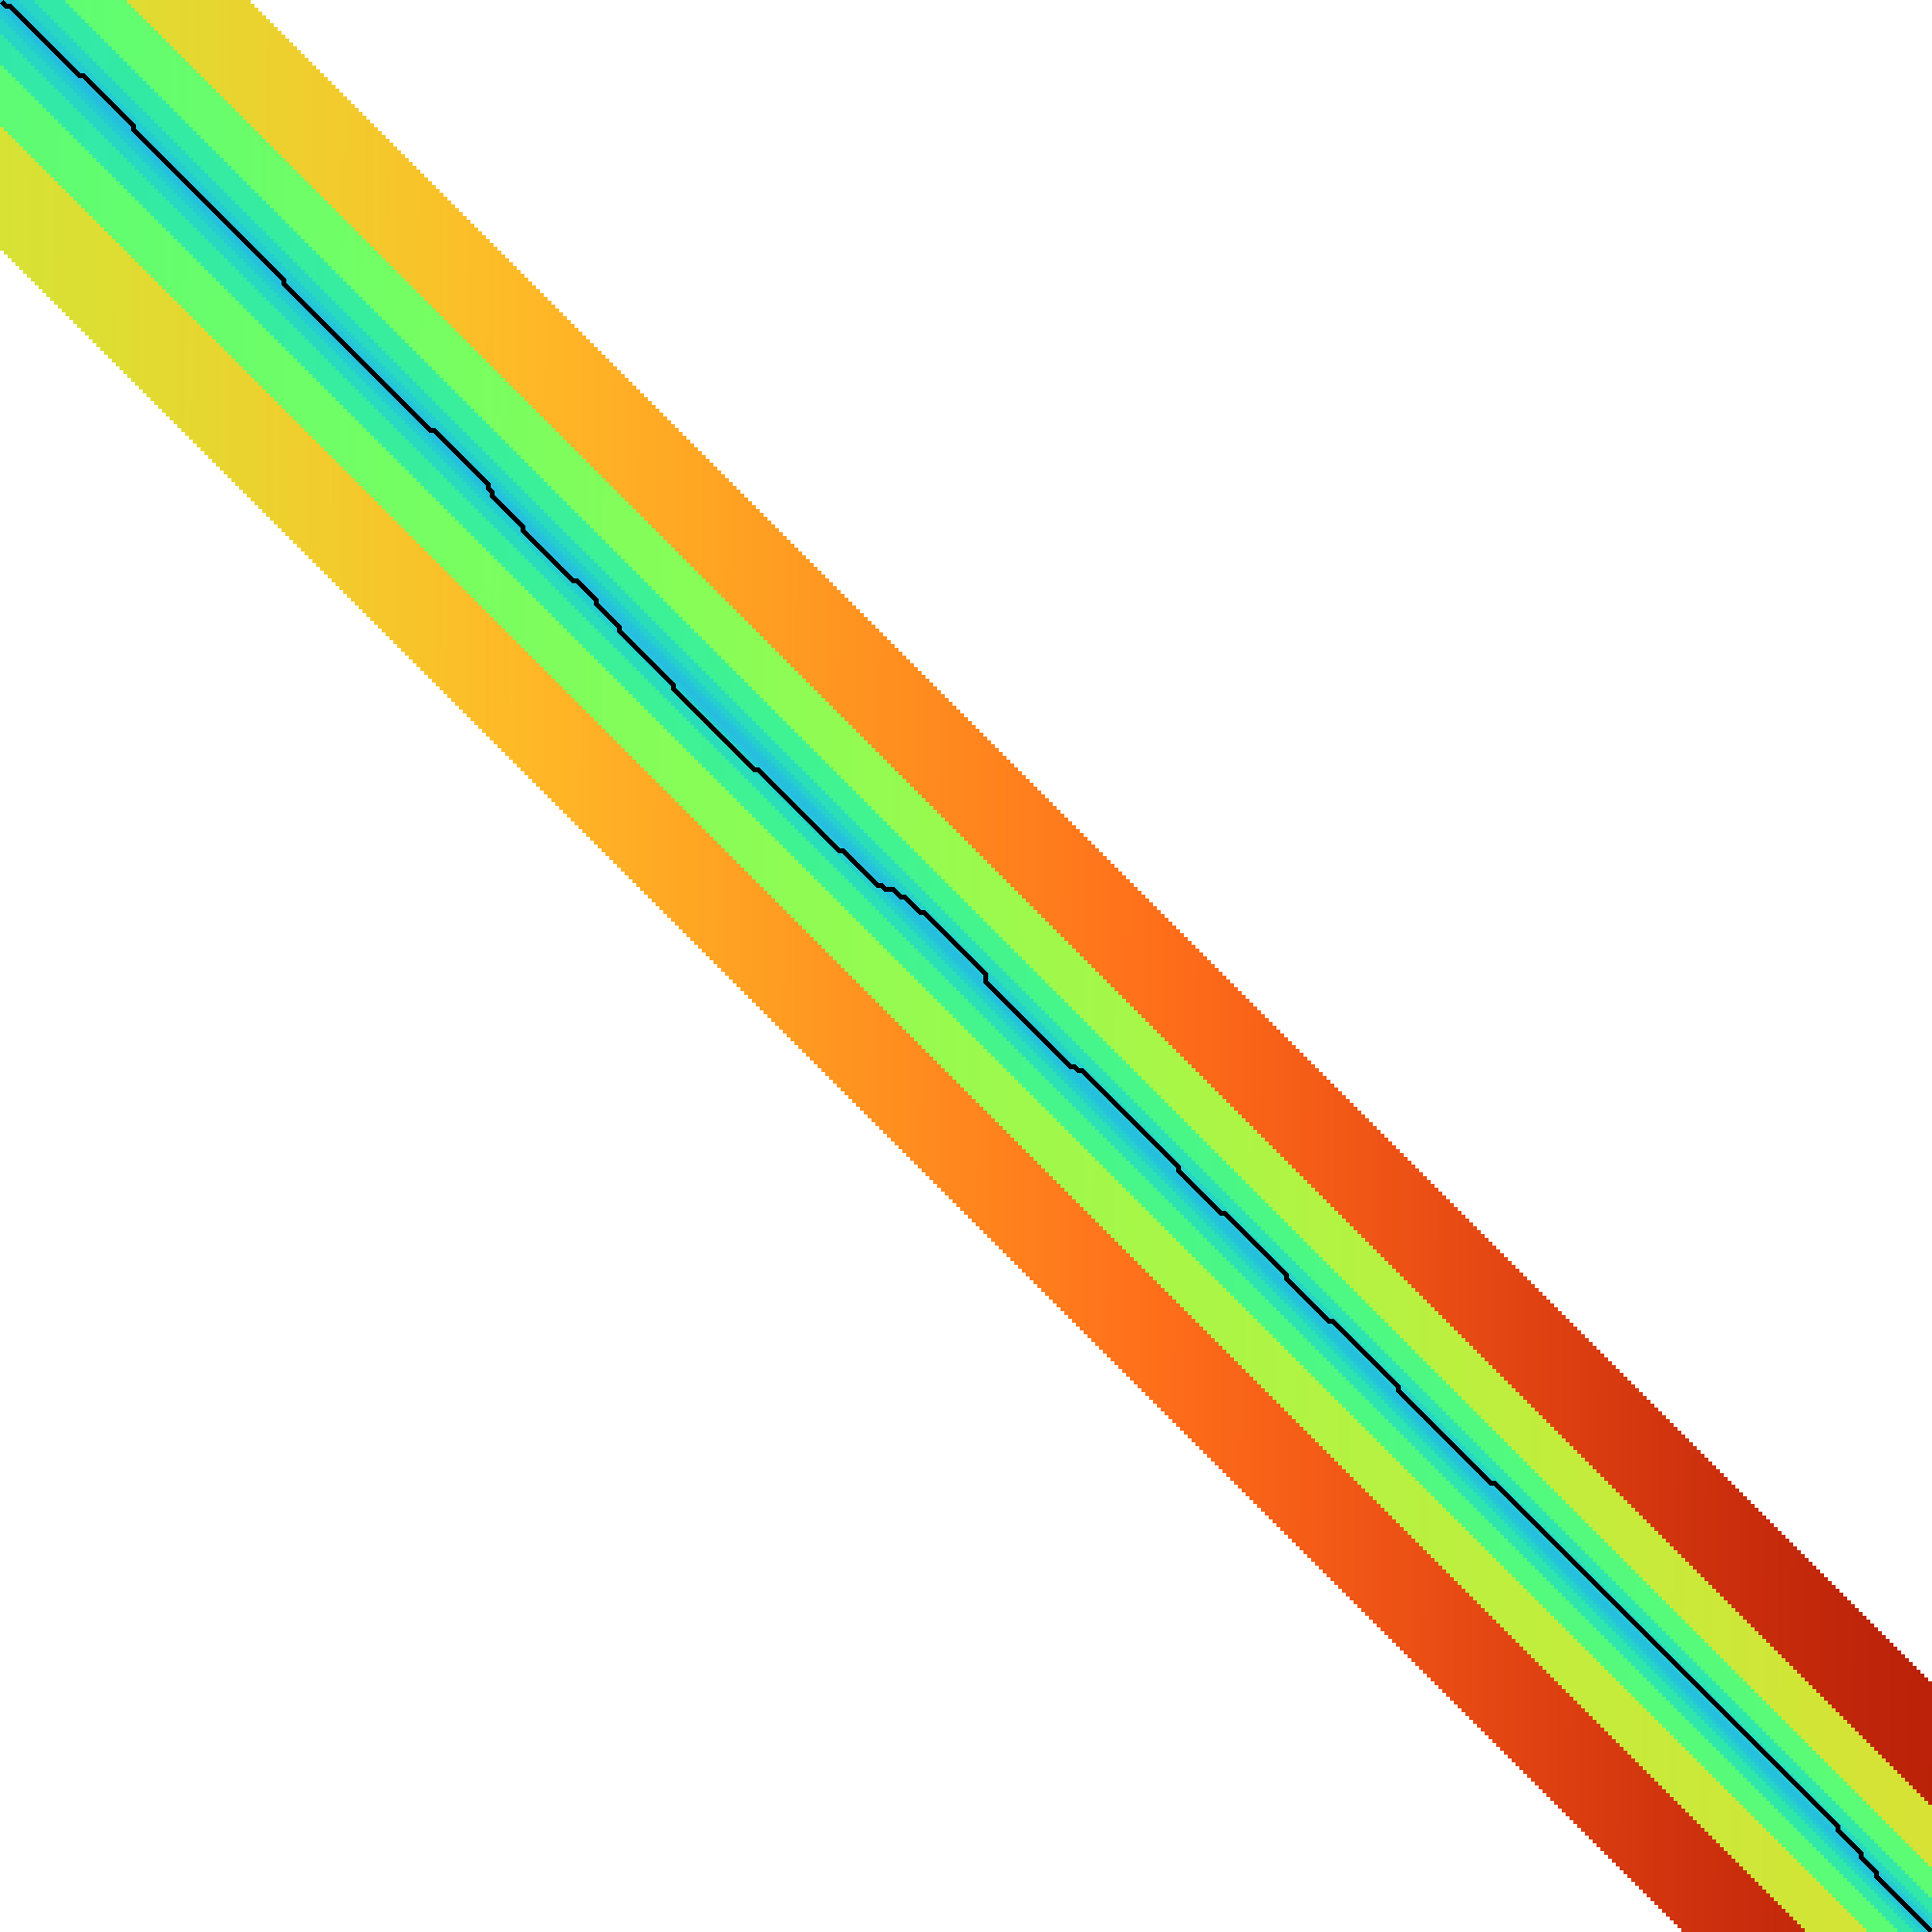
\includegraphics[width=0.3\linewidth]{imgs/fig1/1_ukkonen.png}\label{GLOBALfig1-band}}
    \hspace{-8em}
    \hspace{2.5em}
    \subfloat[\\\dijkstra] {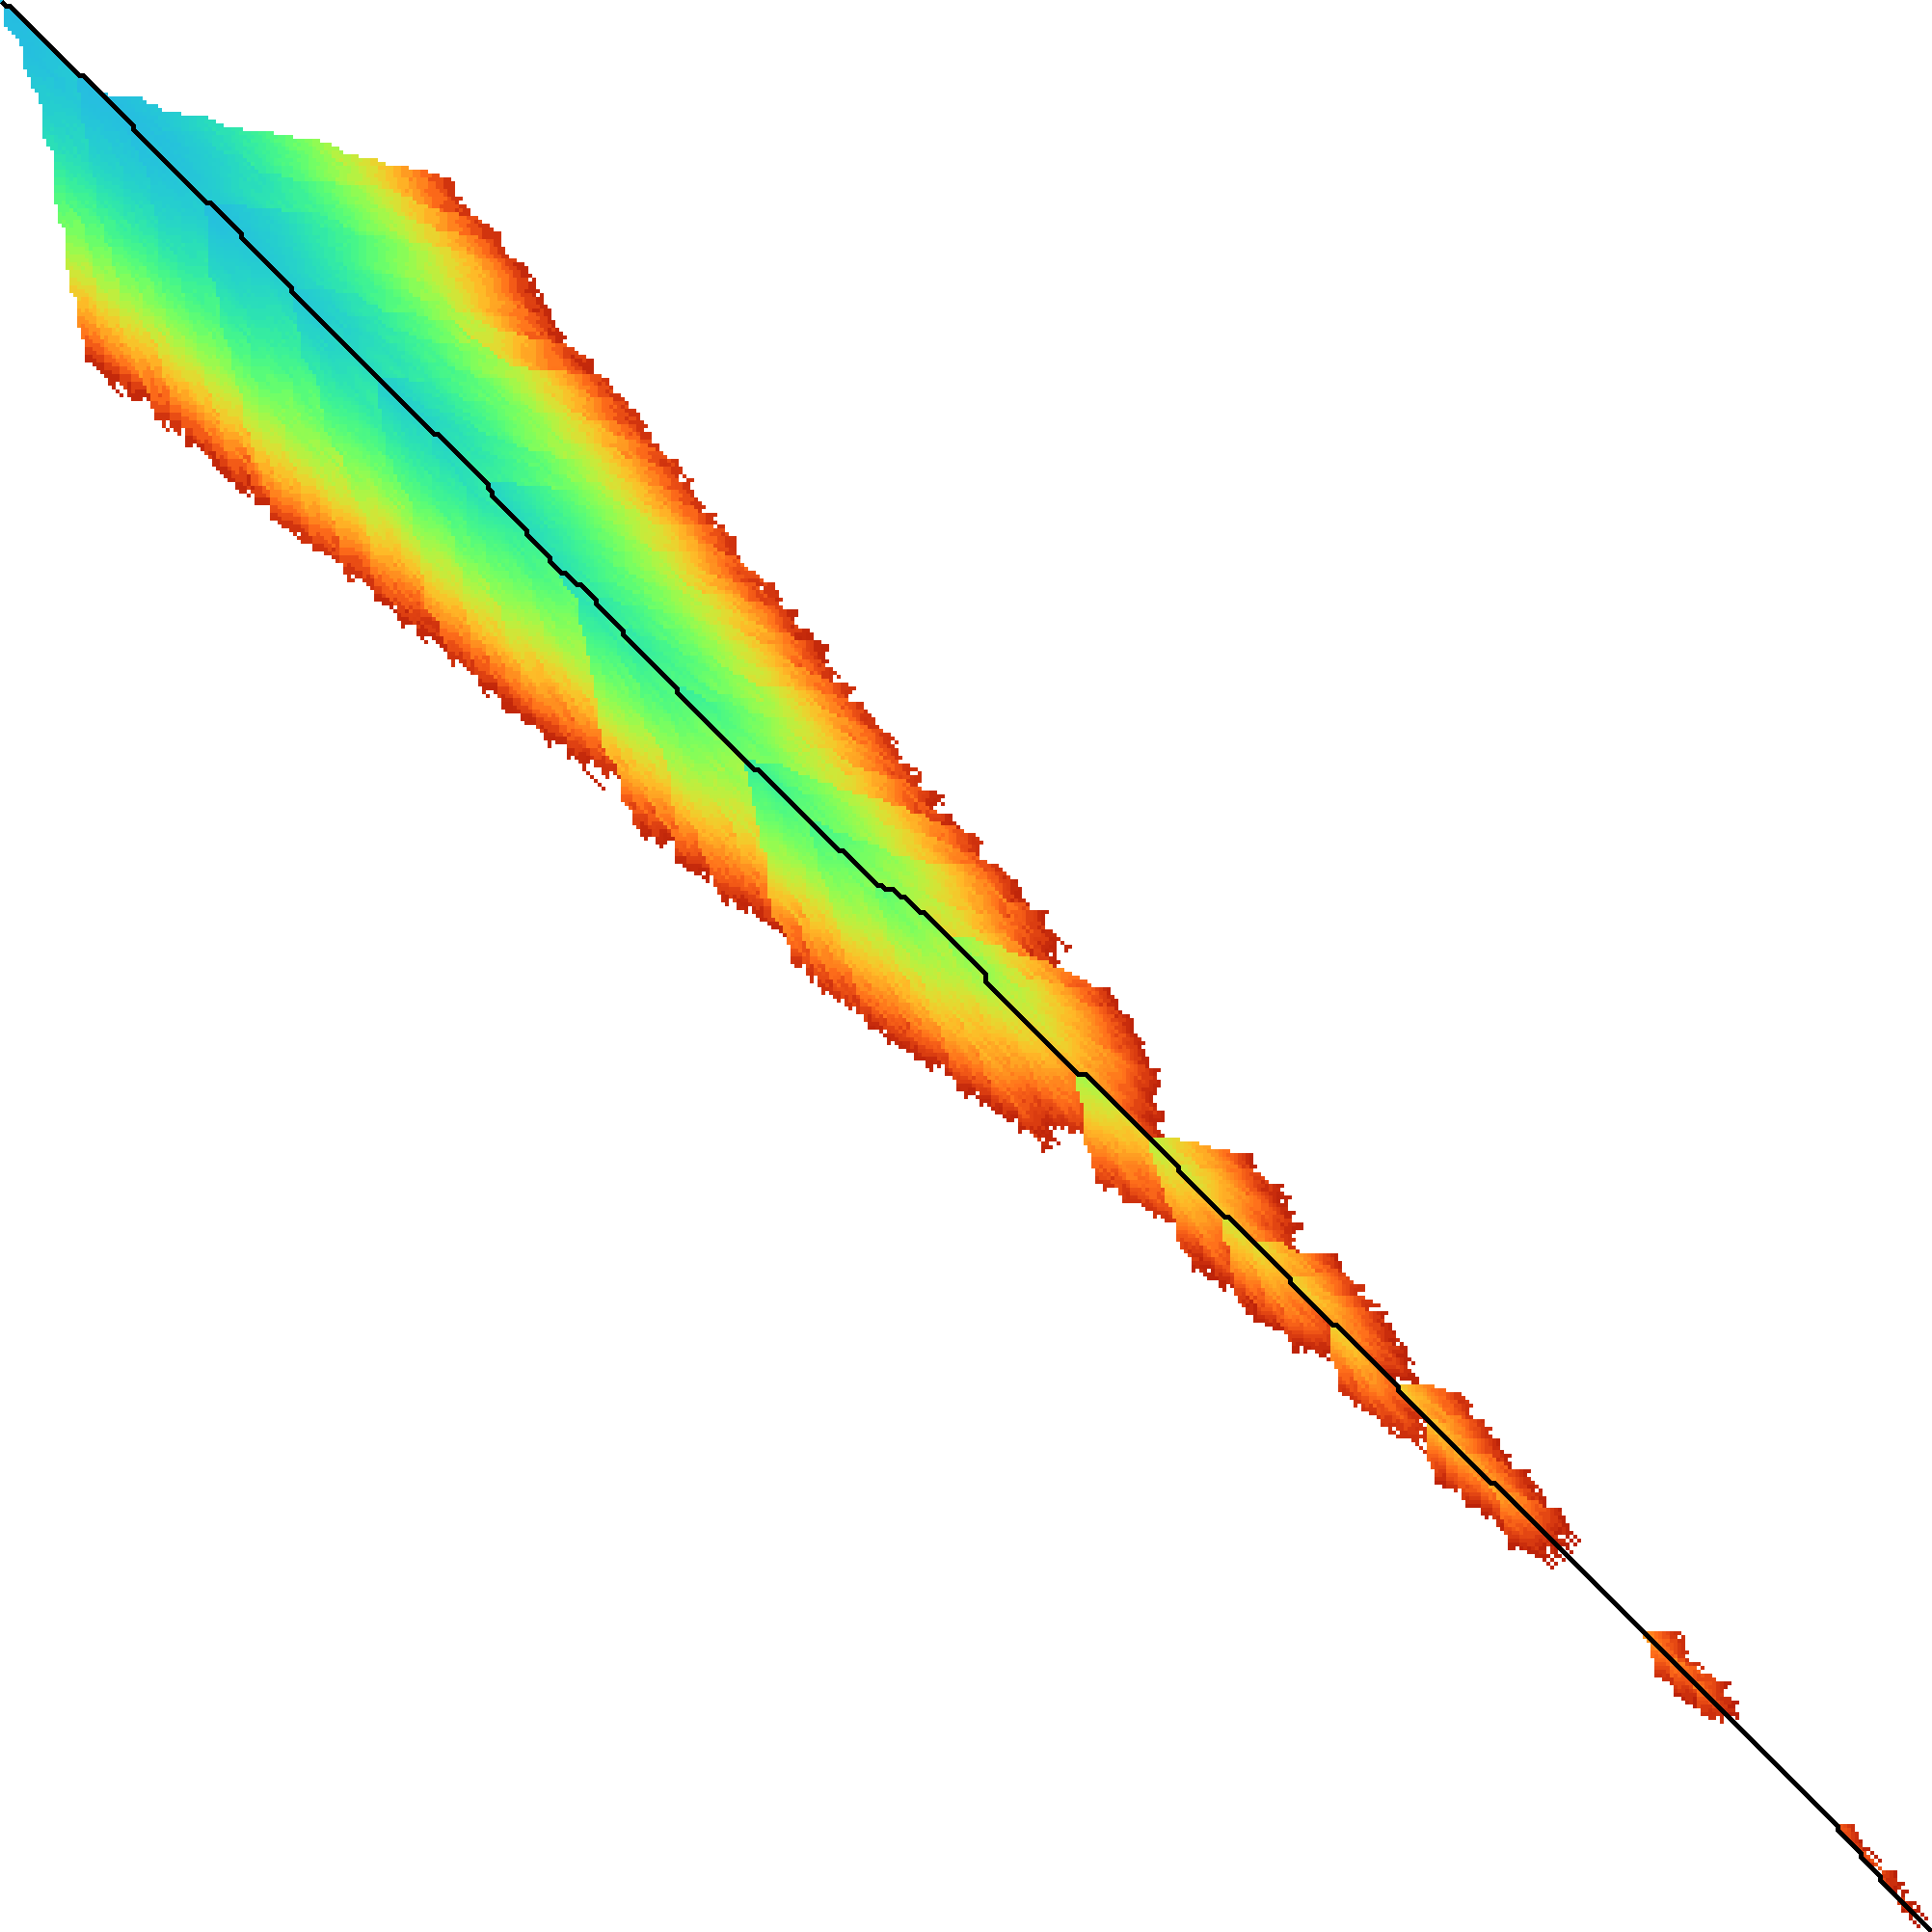
\includegraphics[width=0.3\linewidth]{imgs/fig1/2_dijkstra.png}\label{GLOBALfig1-dij}}
    \hspace{-8em}
    \hspace{2.5em}
    \subfloat[\\DT\\(\oldwfa)]{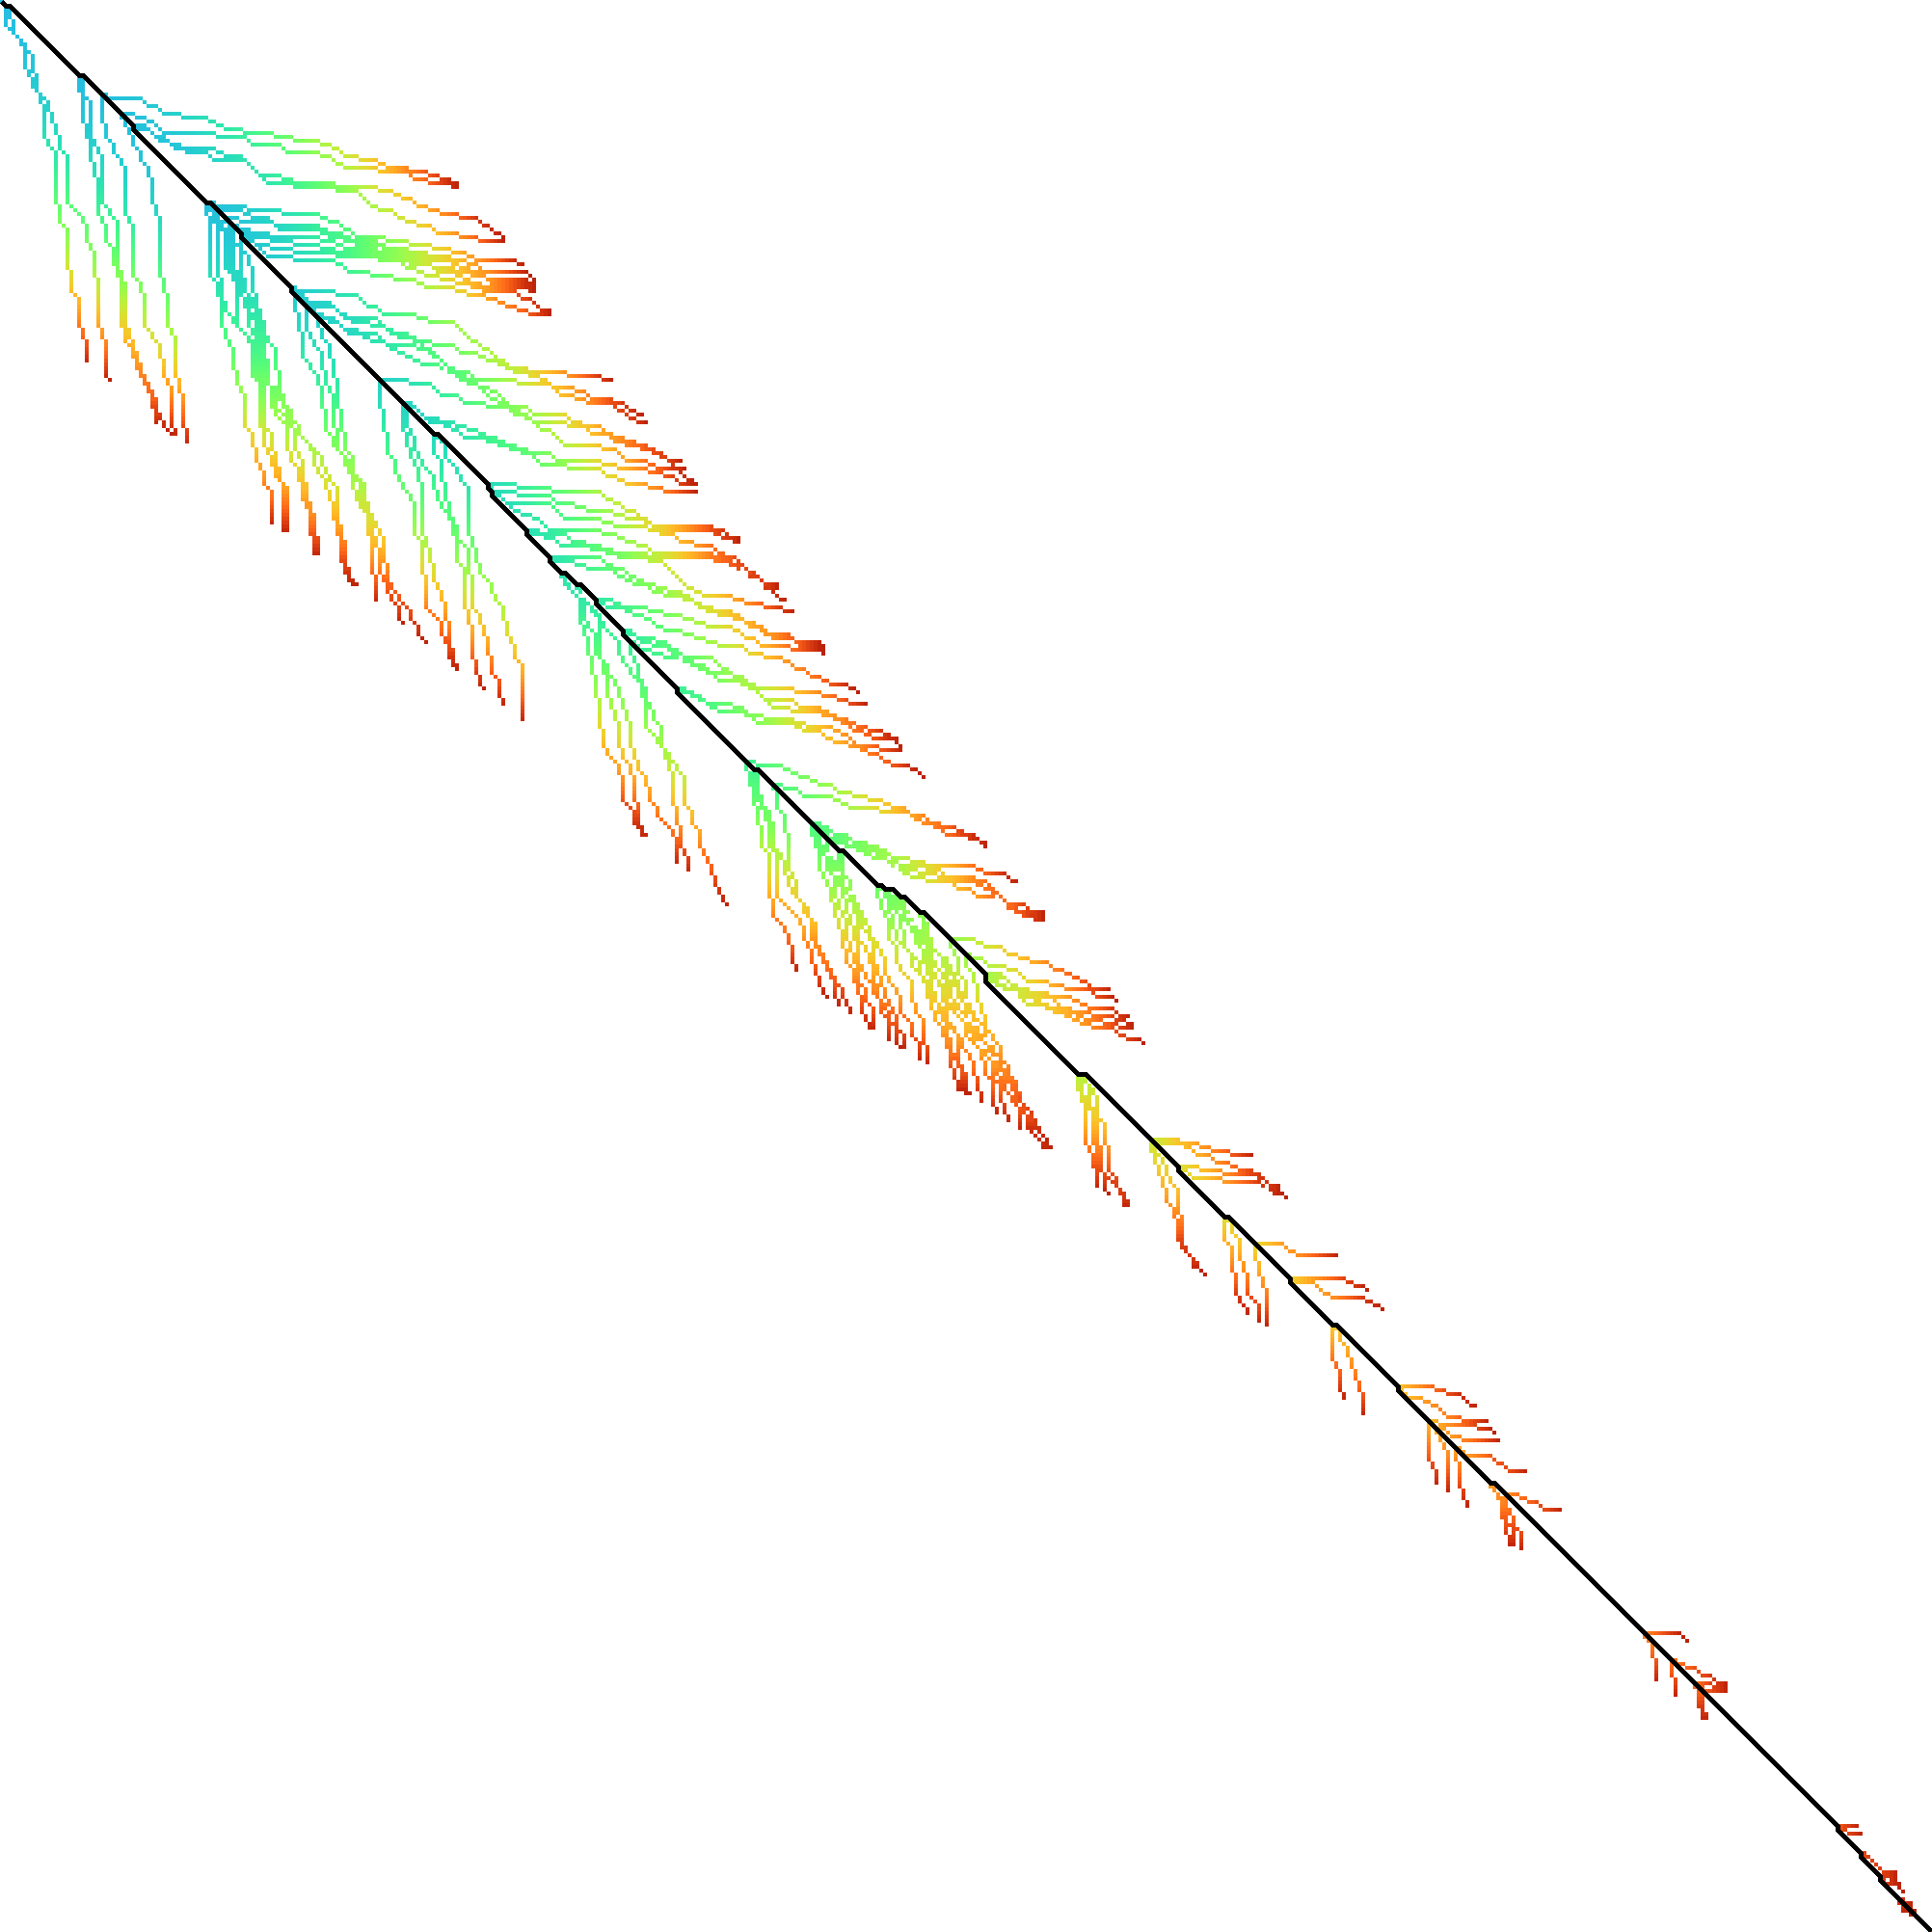
\includegraphics[width=0.3\linewidth]{imgs/fig1/3_diagonal-transition.png}\label{GLOBALfig1-wfa}}
    \hspace{-8em}
    \hspace{2.5em}
    \subfloat[\\DT+D\&C\\(\wfa)]{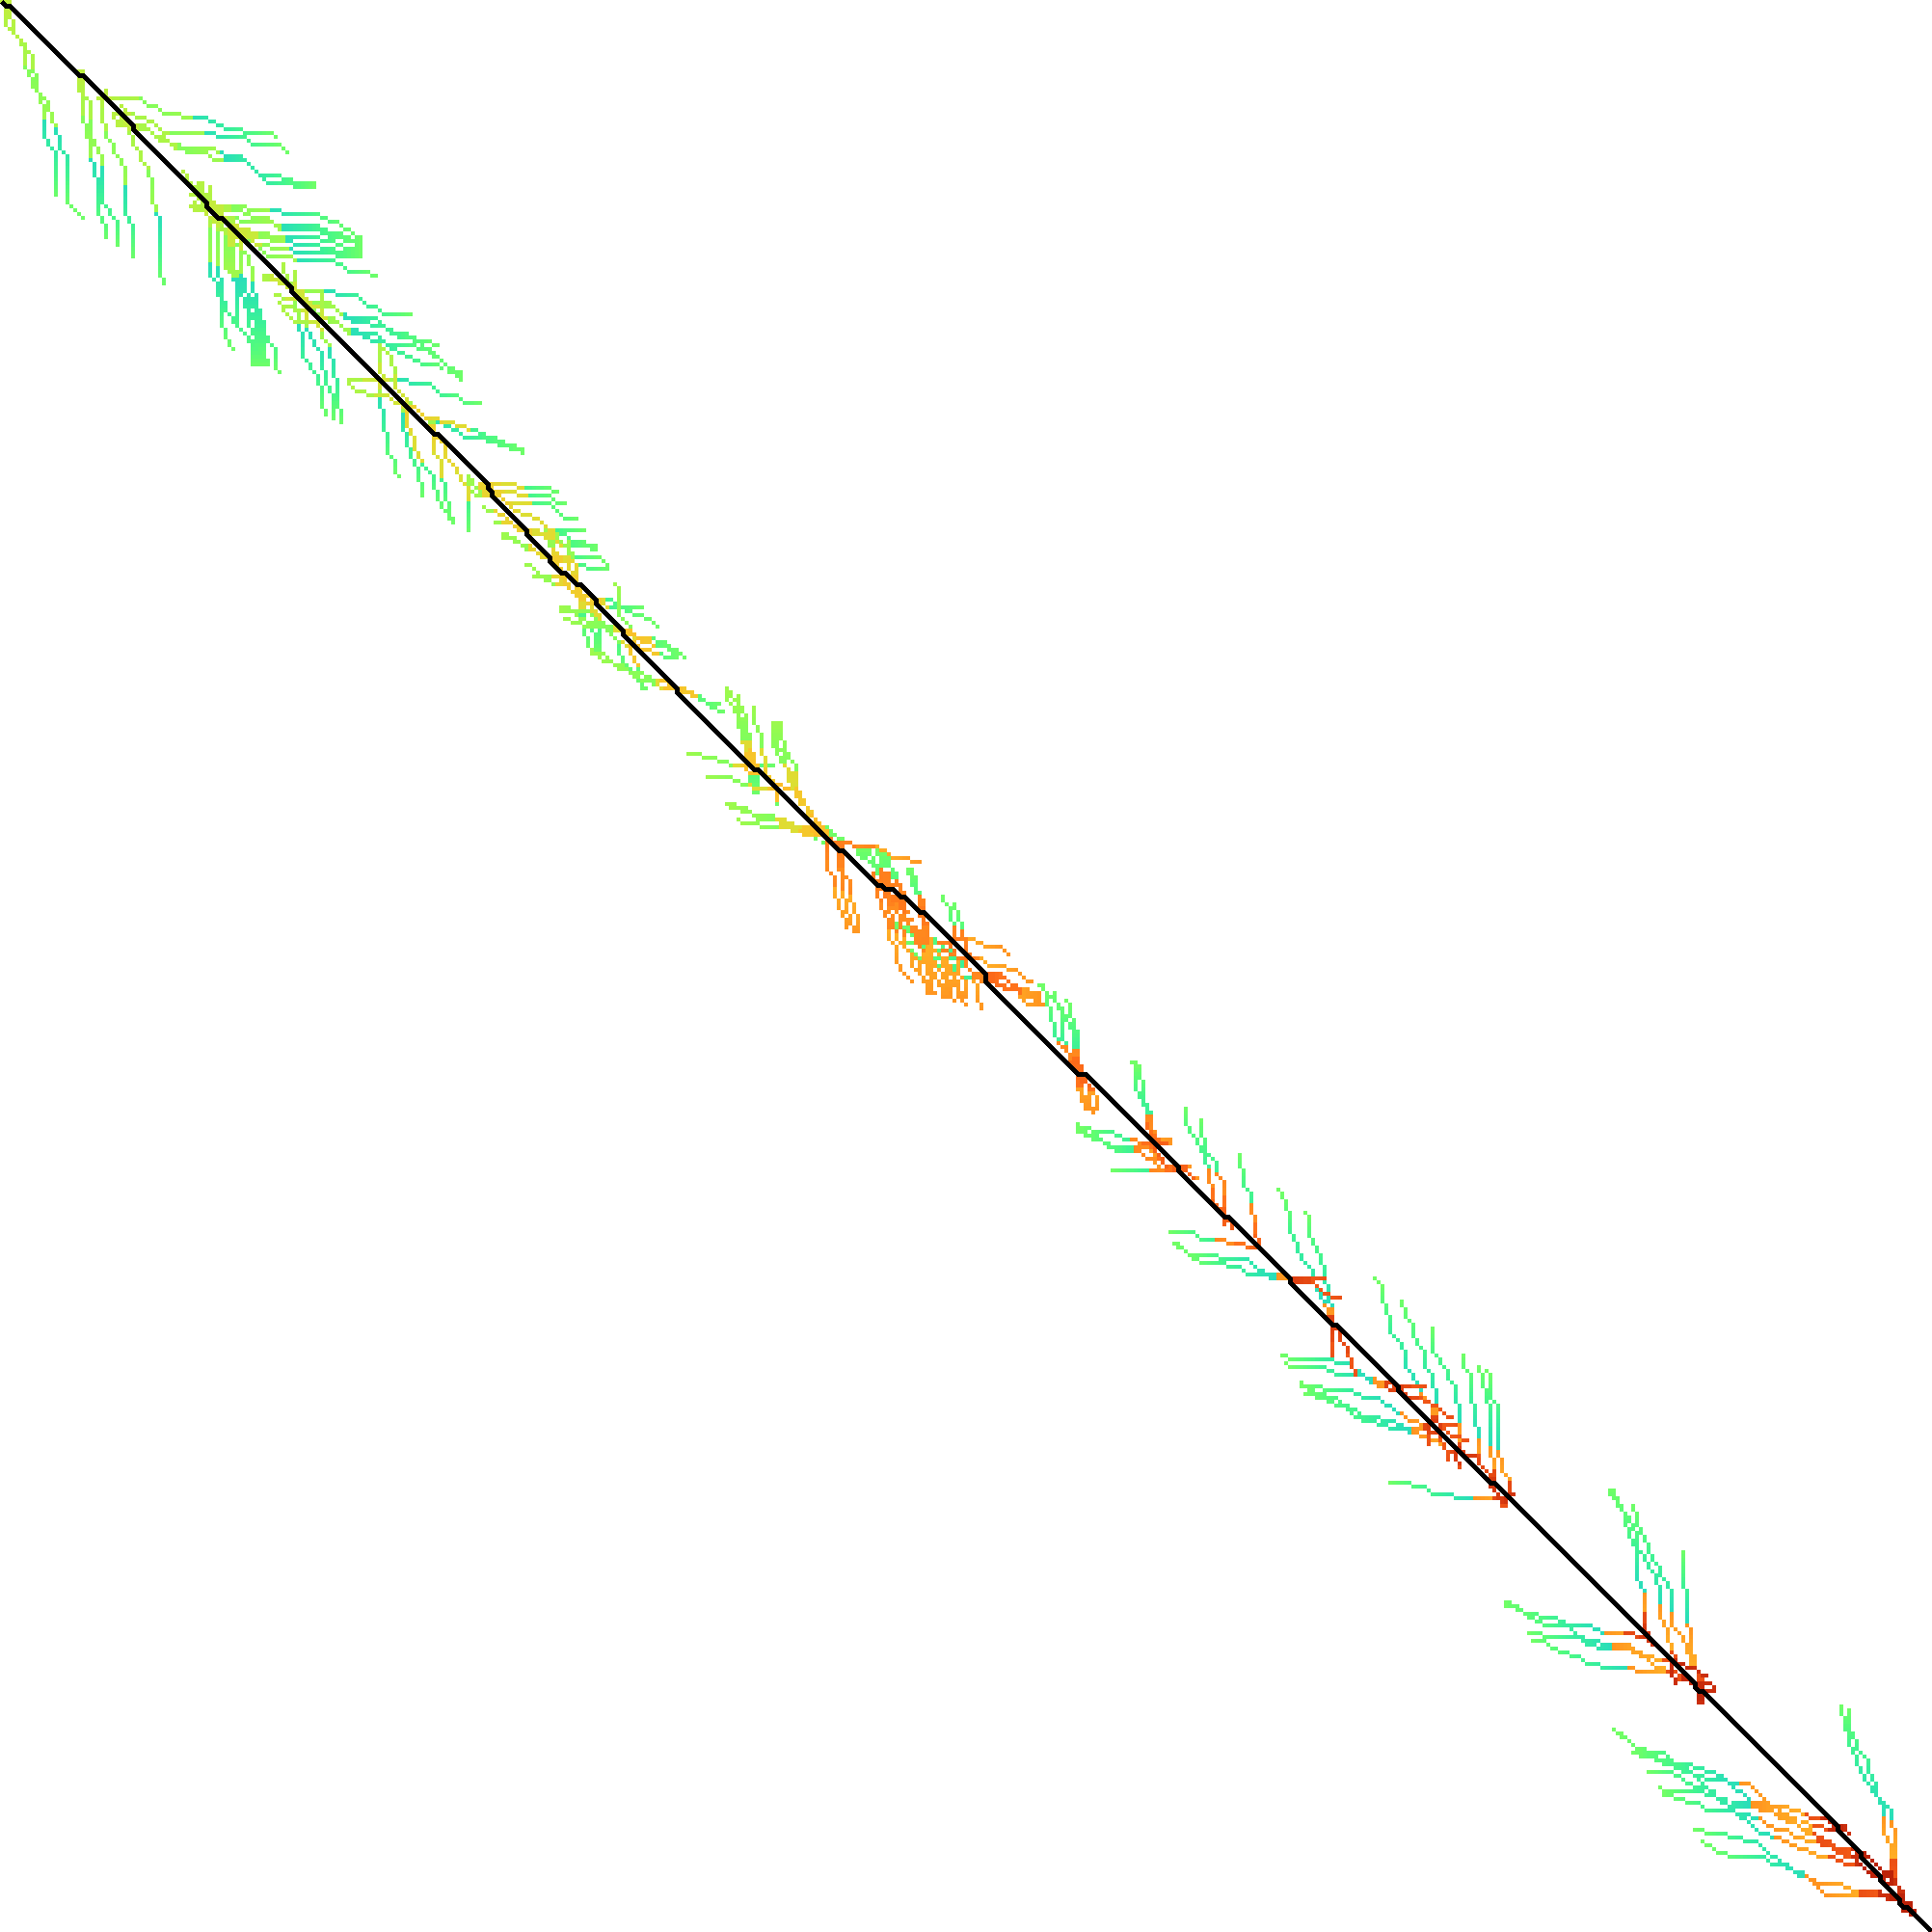
\includegraphics[width=0.3\linewidth]{imgs/fig1/4_dt-divide-and-conquer.png}\label{GLOBALfig1-biwfa}}
    \hspace{-8em}
    \hspace{2.5em}
    \subfloat[\\\textbf{This
    work}\\\textbf{(\astarpa)}]{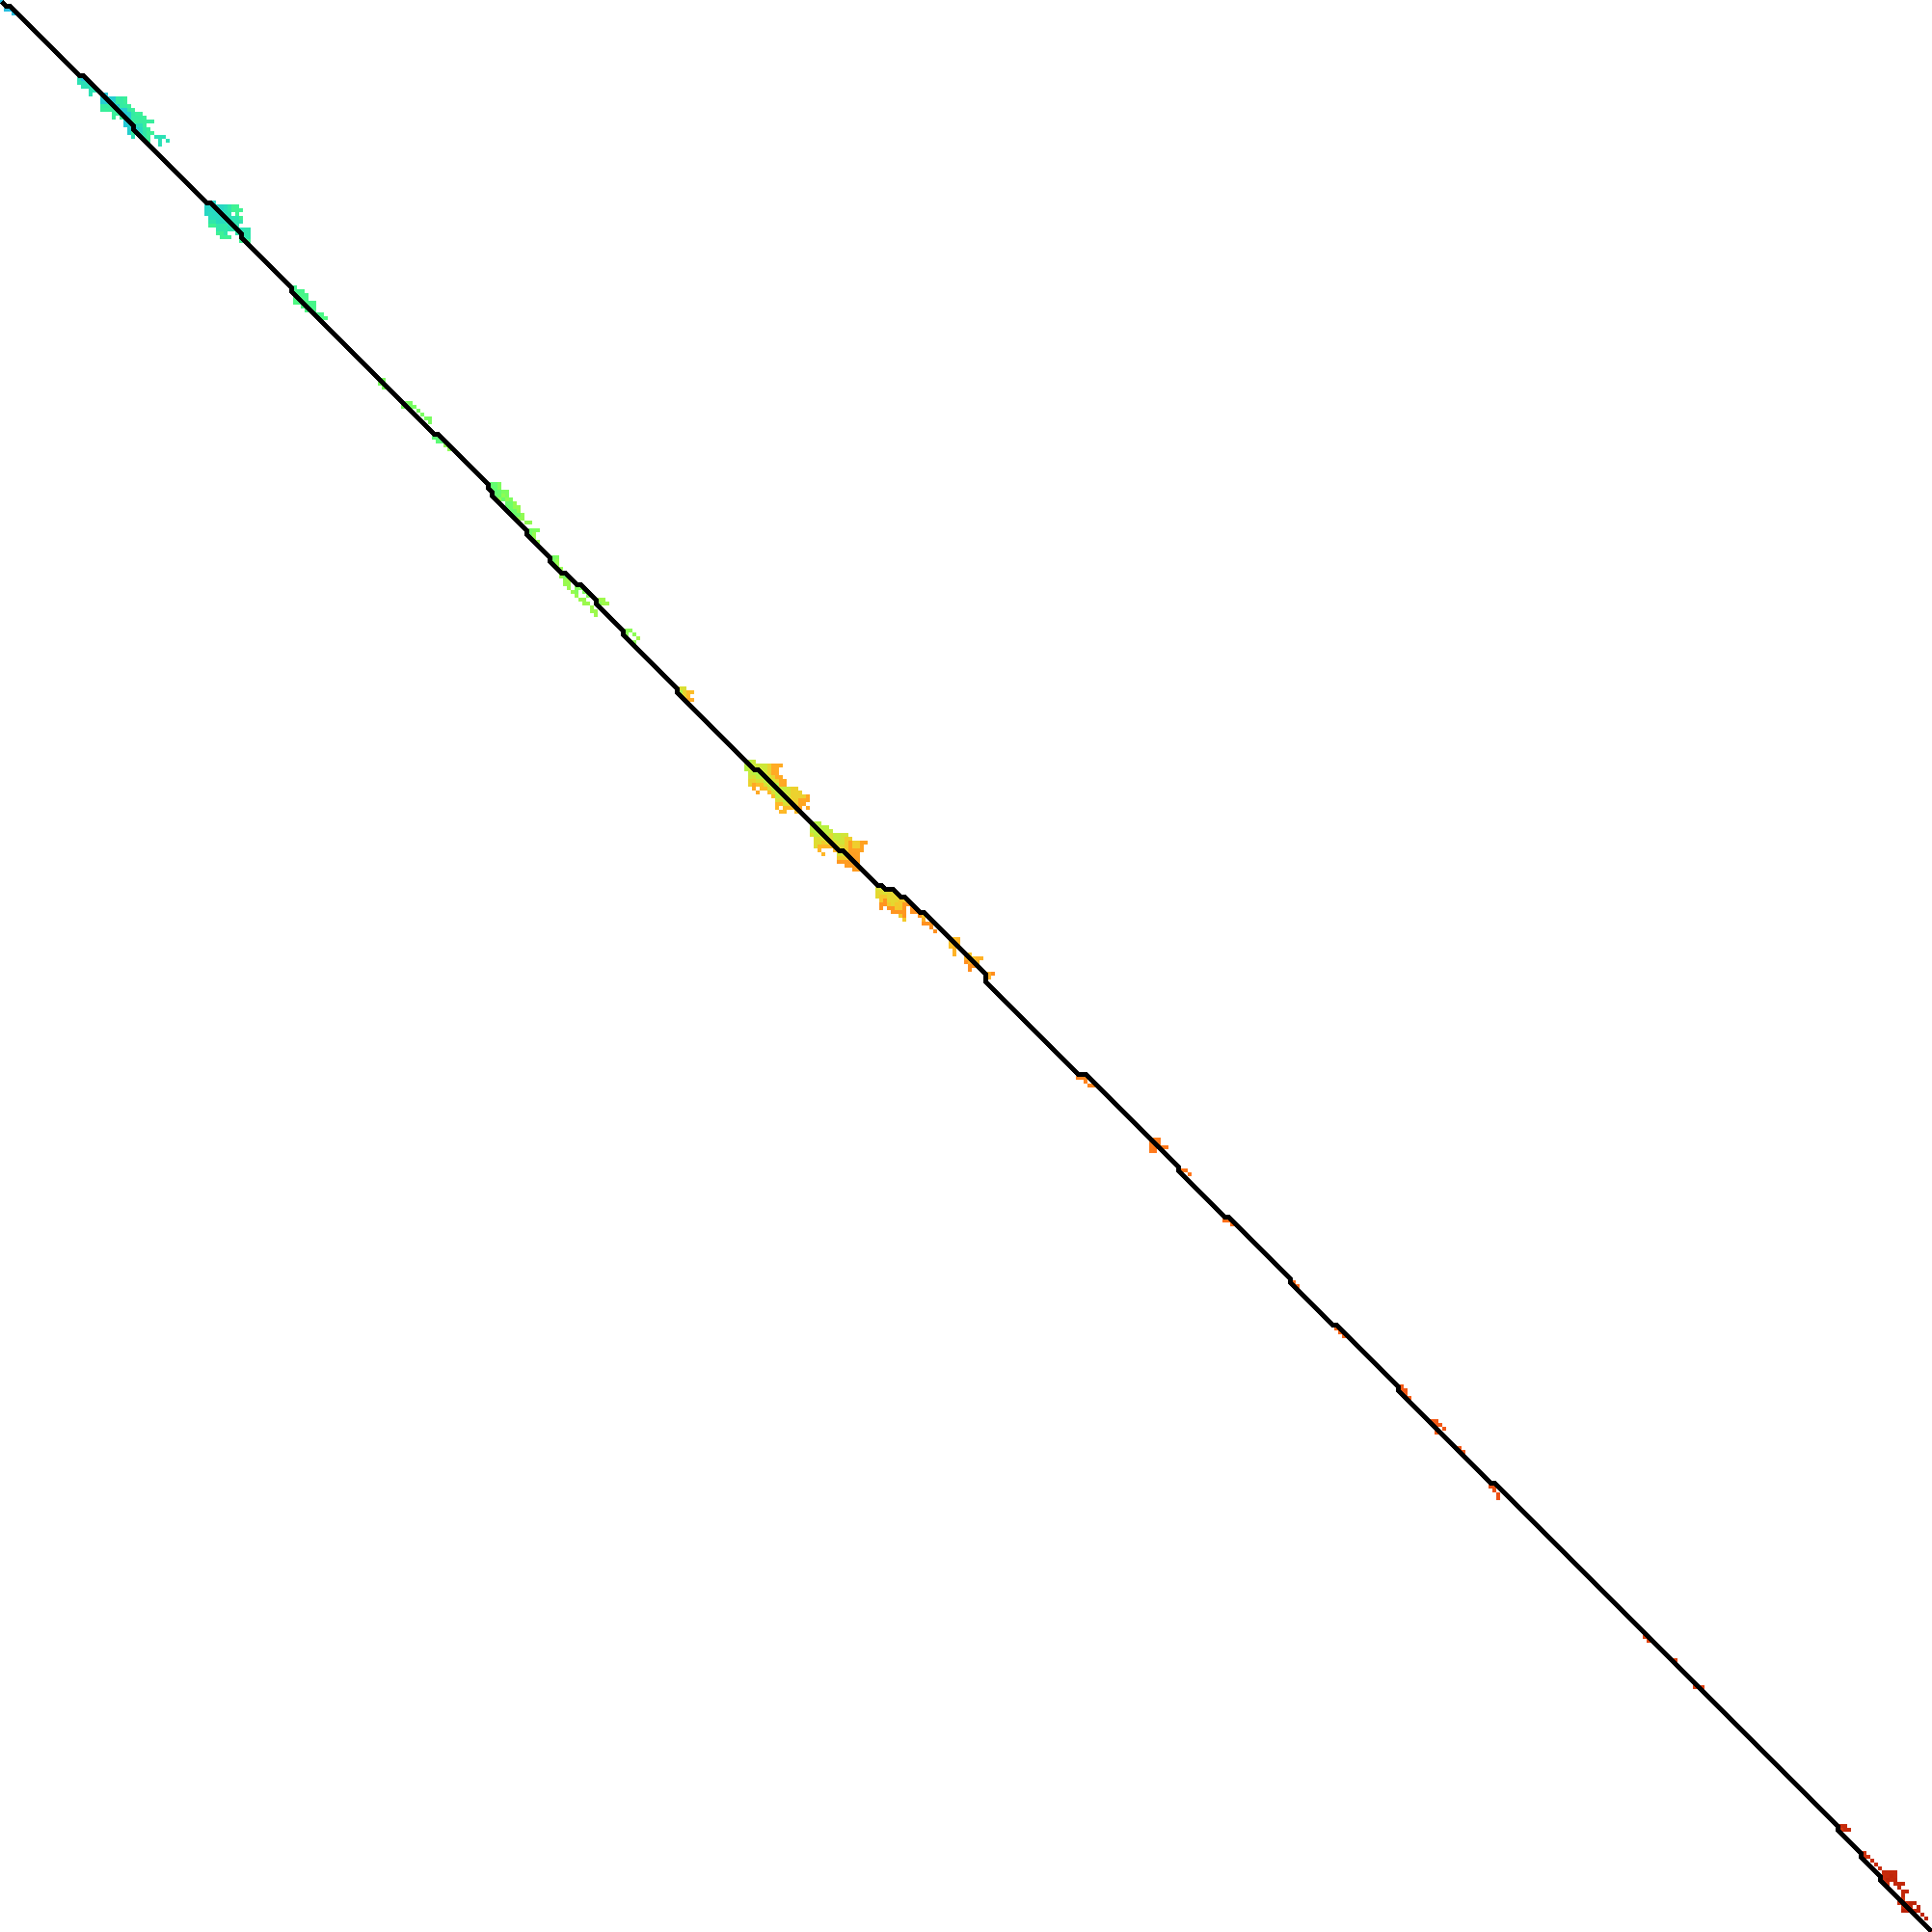
\includegraphics[width=0.3\linewidth]{imgs/fig1/5_astar-csh-pruning.png}\label{GLOBALfig1-astar}}
    \caption[Behavior of various global alignment algorithms]{%
      Demonstration of the computed states by various optimal alignment
algorithms and corresponding aligners that implement them on synthetic data
(length $n{=}500\bp$, error rate $e{=}20\%$). Blue-to-red coloring indicates the
order of computation. \protect\subref{GLOBALfig1-band} Exponential banding
algorithm (\edlib), \protect\subref{GLOBALfig1-dij} \dijkstra,
\protect\subref{GLOBALfig1-wfa} Diagonal transition/DT (\oldwfa),
\protect\subref{GLOBALfig1-biwfa} Diagonal transition with
divide-and-conquer/D\&C (\wfa), \protect\subref{GLOBALfig1-astar} \A with \csh
and match pruning (seed length $k{=}5$ and exact matches). This figure is
produced by Ragnar~Groot Koerkamp and Mykola~Akulov.}
    \label{GLOBALfig:comparison}
\end{figure}
